\hypertarget{part-2-image-3}{%
\section{Part 2, Image 3}\label{part-1-design-2}}

\centering


\hypertarget{description}{%
	\subsubsection{Description}\label{description}}

\begin{description}
	\item[Image:]
	\item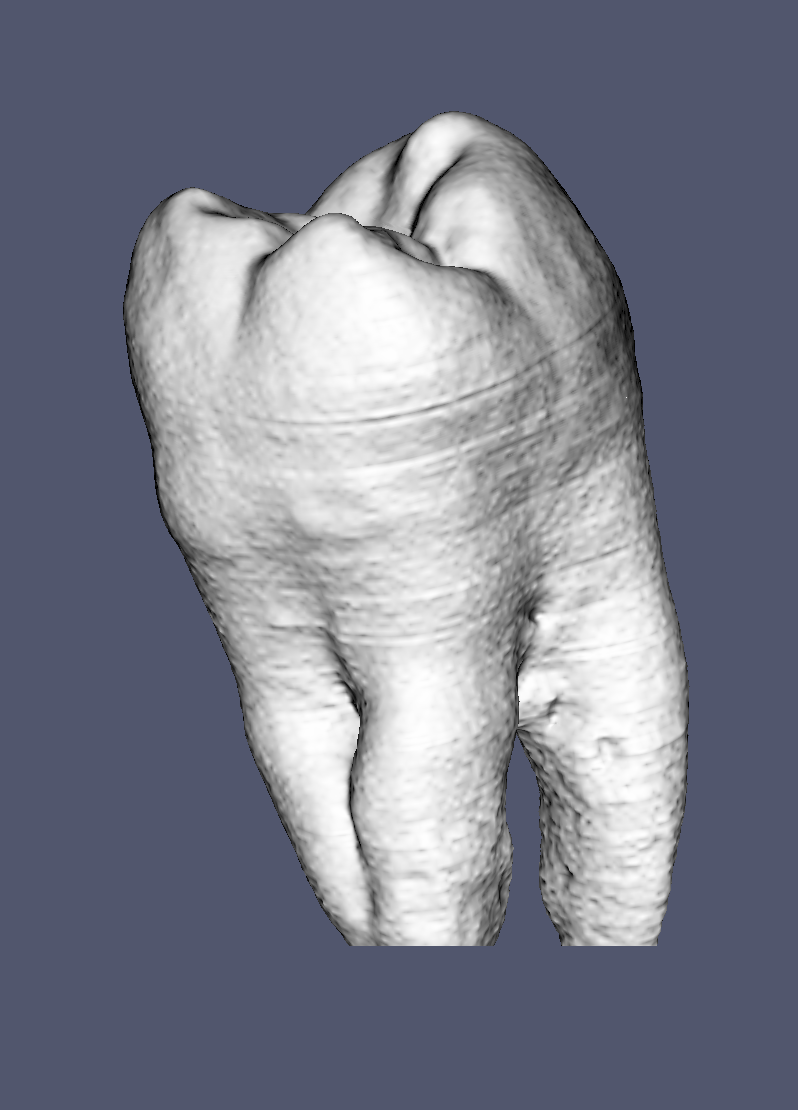
\includegraphics[width=9cm]{Tooth3.png}
		\begin{flushleft}
	\item[Tool:]
	Paraview
	\item[Visual Mappings:]
	\begin{itemize}
		\tightlist
		\item[ ]
	\end{itemize}
	\begin{itemize}
		\tightlist
		\item
		\textbf{mapping 1}: Colour is set to X-ray.
	\end{itemize}
	
	\begin{itemize}
		\tightlist
		\item
		\textbf{mapping 2}: Volume rendering mode is set to OSPRay Based with a blend mode of Isosurface
	\end{itemize}
	\item[Data Conversion:] Data scalar type unsigned char was used. Along with data extent: 0 - 511, 0 - 511, 0 - 181
	\item[Unique Observation:]
	Once the mapping has been altered a tree with leaves appears.

\end{flushleft}	
\end{description}